\chapter{Operating system interfaces}
\label{CH:UNIX}

The job of an operating system is to share a computer among
multiple programs and to provide a more useful set of services
than the hardware alone supports.
An operating system manages and abstracts
the low-level hardware, so that, for example,
a word processor need not concern itself with which type
of disk hardware is being used.
An operating system shares the hardware among multiple programs so
that they run (or appear to run) at the same time.
Finally, operating systems provide controlled ways for programs
to interact, so that they can share data or work together.

An operating system provides services to user programs through an interface.
\index{interface design}
Designing a good interface turns out to be
difficult.  On the one hand, we would like the interface to be
simple and narrow because that makes it easier to get the
implementation right.  On the other hand,
we may be tempted to offer many sophisticated features to applications.
The trick in
resolving this tension is to design interfaces that rely on a few
mechanisms that can be combined to provide much generality.

This book uses a single operating system as a concrete example to
illustrate operating system concepts.  That operating system,
xv6, provides the basic interfaces introduced by Ken Thompson and
Dennis Ritchie's Unix operating system~\cite{unix}, as well as mimicking Unix's
internal design.  Unix provides a
narrow interface whose mechanisms combine well, offering a surprising
degree of generality.  This interface has been so successful that
modern operating systems—BSD, Linux, Mac OS X, Solaris, and even, to a
lesser extent, Microsoft Windows—have Unix-like interfaces.
Understanding xv6 is a good start toward understanding any of these
systems and many others.

As 
Figure~\ref{fig:os} shows,
xv6 takes the traditional form of a
\indextext{kernel},
a special program that provides
services to running programs.
Each running program, called a
\indextext{process},
has memory containing instructions, data, and a stack. The
instructions implement the
program's computation.  The data are the variables on which
the computation acts. The stack organizes the program's procedure calls.
A given computer typically has many processes but only a single
kernel.

When a
process needs to invoke a kernel service, it invokes 
a \indextext{system call},
one of the calls
in the operating system's interface.
The system call enters the kernel;
the kernel performs the service and returns.
Thus a process alternates between executing in
\indextext{user space}
and
\indextext{kernel space}.

The kernel uses the hardware protection mechanisms provided by a
CPU\footnote{
This text generally refers to the hardware element that executes a
computation with the term \indextext{CPU}, an acronym for central
processing unit.  Other documentation (e.g., the RISC-V specification)
also uses the words processor, core, and hart instead of CPU.
}
to
ensure that each process executing in user space can access only
its own memory.
The kernel executes with the hardware privileges required to
implement these protections; user programs execute without
those privileges.
When a user program invokes a system call, the hardware
raises the privilege level and starts executing a pre-arranged
function in the kernel.

\begin{figure}[t]
\center
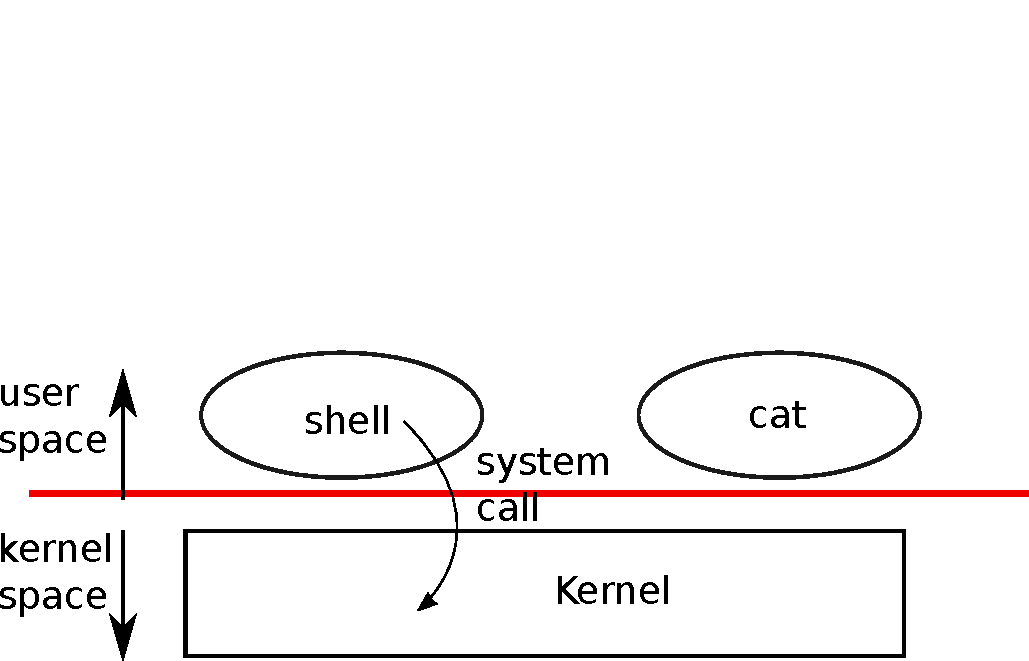
\includegraphics[scale=0.5]{fig/os.pdf}
\caption{A kernel and two user processes.}
\label{fig:os}
\end{figure}

The collection of system calls that a kernel provides
is the interface that user programs see.
The xv6 kernel provides a subset of the services and system calls
that Unix kernels traditionally offer.  
Figure~\ref{fig:api} 
lists all of xv6's system calls.

The rest of this chapter outlines xv6's services---processes, memory,
file descriptors, pipes, and a file system---and illustrates them with
code snippets and discussions of how the \indextext{shell}, 
Unix's command-line user interface, uses
them. The shell's use of system calls illustrates how carefully they
have been designed.

The shell is an ordinary program that reads commands from the user
and executes them.
The fact that the shell is a user program, and not part of the kernel,
illustrates the power of the system call interface: there is nothing
special about the shell.
It also means that the shell is easy to replace; as a result,
modern Unix systems have a variety of
shells to choose from, each with its own user interface
and scripting features.
The xv6 shell is a simple implementation of the essence of
the Unix Bourne shell.  Its implementation can be found at 
\lineref{user/sh.c:1}.
%% 
%% 	Processes and memory
%% 
\section{Processes and memory}

An xv6 process consists of user-space memory (instructions, data, and stack)
and per-process state private to the kernel.
Xv6 
\indextext{time-share}s
processes: it transparently switches the available CPUs
among the set of processes waiting to execute.
When a process is not executing, xv6 saves its CPU registers,
restoring them when it next runs the process.
The kernel associates a process identifier, or
\indexcode{PID},
with each process.

\begin{figure}[t]
\center
\begin{tabular}{ll}
{\bf System call} & {\bf Description} \\
\midrule
int fork() & Create a process, return child's PID. \\
int exit(int status) & Terminate the current process; status reported to wait(). No return. \\
int wait(int *status) & Wait for a child to exit; exit status in *status; returns child PID. \\
int kill(int pid) & Terminate process PID. Returns 0, or -1 for error. \\
int getpid() & Return the current process's PID. \\
int sleep(int n) & Pause for n clock ticks. \\
int exec(char *file, char *argv[]) & Load a file and execute it with arguments; only returns if error. \\
char *sbrk(int n) & Grow process's memory by n bytes. Returns start of new memory. \\
int open(char *file, int flags) & Open a file; flags indicate read/write; returns an fd (file descriptor). \\
int write(int fd, char *buf, int n) & Write n bytes from buf to file descriptor fd; returns n. \\
int read(int fd, char *buf, int n) & Read n bytes into buf; returns number read; or 0 if end of file. \\
int close(int fd) & Release open file fd. \\
int dup(int fd) & Return a new file descriptor referring to the same file as fd.\\
int pipe(int p[]) & Create a pipe, put read/write file descriptors in p[0] and p[1]. \\
int chdir(char *dir) & Change the current directory. \\
int mkdir(char *dir) & Create a new directory. \\
int mknod(char *file, int, int) & Create a device file. \\
int fstat(int fd, struct stat *st) & Return info about an open file. \\
int stat(char *file, struct stat *st) & Return info about a named file. \\
int link(char *file1, char *file2) & Create another name (file2) for the file file1. \\
int unlink(char *file) & Remove a file. \\
\end{tabular}
\caption{Xv6 system calls. If not otherwise stated, these calls return
0 for no error, and -1 if there's an error.}
\label{fig:api}
\end{figure}

A process may create a new process using the
\indexcode{fork}
system call.
\lstinline{Fork}
creates a new process, called the 
\indextext{child process}, 
with exactly the same memory contents
as the calling process, called the 
\indextext{parent process}.
\lstinline{Fork}
returns in both the parent and the child.
In the parent,
\indexcode{fork}
returns the child's PID;
in the child, \lstinline{fork} returns zero.
For example, consider the following program fragment written in the C
programming language~\cite{kernighan}:
\begin{lstlisting}[]
int pid = fork();
if(pid > 0){
  printf("parent: child=%d\n", pid);
  pid = wait((int *) 0);
  printf("child %d is done\n", pid);
} else if(pid == 0){
  printf("child: exiting\n");
  exit(0);
} else {
  printf("fork error\n");
}
\end{lstlisting}
The
\indexcode{exit}
system call causes the calling process to stop executing and
to release resources such as memory and open files.
Exit takes an integer status argument,
conventionally 0 to indicate success and 1 to indicate failure.
The
\indexcode{wait}
system call returns the PID of an exited (or killed) child of the
current process and copies the exit status of the child to the address
passed to wait; if none of the caller's children
has exited,
\indexcode{wait}
waits for one to do so.
If the caller has no children, \lstinline{wait} immediately
returns -1.
If the parent doesn't care about the exit status of a child, it can
pass a 0 address to
\lstinline{wait}.

In the example, the output lines
\begin{lstlisting}[]
parent: child=1234
child: exiting
\end{lstlisting}
might come out in either order, depending on whether the
parent or child gets to its
\indexcode{printf}
call first.
After the child exits, the parent's
\indexcode{wait}
returns, causing the parent to print
\begin{lstlisting}[]
parent: child 1234 is done
\end{lstlisting}
Although the child has the same memory contents as the parent initially, the
parent and child are executing with different memory and different registers:
changing a variable in one does not affect the other. For example, when the
return value of
\lstinline{wait}
is stored into
\lstinline{pid} 
in the parent process,
it doesn't change the variable 
\lstinline{pid}
in the child.  The value of
\lstinline{pid}
in the child will still be zero.

The
\indexcode{exec}
system call
replaces the calling process's memory with a new memory
image loaded from a file stored in the file system.
The file must have a particular format, which specifies which part of
the file holds instructions, which part is data, at which instruction
to start, etc. xv6
uses the ELF format, which Chapter~\ref{CH:MEM} discusses in
more detail.
When
\indexcode{exec}
succeeds, it does not return to the calling program;
instead, the instructions loaded from the file start
executing at the entry point declared in the ELF header.
\lstinline{Exec}
takes two arguments: the name of the file containing the
executable and an array of string arguments.
For example:
\begin{lstlisting}[]
char *argv[3];

argv[0] = "echo";
argv[1] = "hello";
argv[2] = 0;
exec("/bin/echo", argv);
printf("exec error\n");
\end{lstlisting}
This fragment replaces the calling program with an instance
of the program 
\lstinline{/bin/echo}
running with the argument list
\lstinline{echo}
\lstinline{hello}.
Most programs ignore the first element of the argument array, which is 
conventionally the name of the program.

The xv6 shell uses the above calls to run programs on behalf of
users. The main structure of the shell is simple; see
\lstinline{main} 
\lineref{user/sh.c:/main/}.
The main loop reads a line of input from the user with
\indexcode{getcmd}.
Then it calls 
\lstinline{fork}, 
which creates a copy of the shell process. The
parent calls
\lstinline{wait},
while the child runs the command.  For example, if the user
had typed
``\lstinline{echo hello}''
to the shell,
\lstinline{runcmd}
would have been called with
``\lstinline{echo hello}''
as the argument.
\lstinline{runcmd} 
\lineref{user/sh.c:/runcmd/}
runs the actual command. For
``\lstinline{echo hello}'',
it would call
\lstinline{exec} 
\lineref{user/sh.c:/exec.ecmd/}.
If
\lstinline{exec}
succeeds then the child will execute instructions from
\lstinline{echo}
instead of
\lstinline{runcmd}.  
At some point
\lstinline{echo}
will call
\lstinline{exit},
which will cause the parent to return from
\lstinline{wait}
in 
\lstinline{main}
\lineref{user/sh.c:/main/}.

You might wonder why
\indexcode{fork}
and
\indexcode{exec}
are not combined in a single call; we will see later that 
the shell exploits the separation in its implementation of
I/O redirection.
To avoid the wastefulness of
creating a duplicate process and then immediately replacing it (with \lstinline{exec}),
operating kernels optimize the implementation of
\lstinline{fork}
for this use case by using virtual memory techniques such as
copy-on-write (see Section~\ref{sec:pagefaults}).

Xv6 allocates most user-space memory
implicitly:
\indexcode{fork}
allocates the memory required for the child's copy of the
parent's memory, and 
\indexcode{exec}
allocates enough memory to hold the executable file.
A process that needs more memory at run-time (perhaps for
\indexcode{malloc})
can call
\lstinline{sbrk(n)}
to grow its data memory by
\lstinline{n}
bytes;
\indexcode{sbrk}
returns the location of the new memory.

%% 
%% 	I/O and File descriptors
%% 
\section{I/O and File descriptors}

A 
\indextext{file descriptor} 
is a small integer representing a kernel-managed object
that a process may read from or write to.
A process may obtain a file descriptor by opening a file, directory,
or device, or by creating a pipe, or by duplicating an existing
descriptor.
For simplicity we'll often refer to the object a file descriptor
refers to as a ``file'';
the file descriptor interface abstracts away the differences between
files, pipes, and devices, making them all look like streams of bytes.
We'll refer to input and output as \indextext{I/O}.

Internally, the xv6 kernel uses the file descriptor
as an index into a per-process table,
so that every process has a private space of file descriptors
starting at zero.
By convention, a process reads from file descriptor 0 (standard input),
writes output to file descriptor 1 (standard output), and
writes error messages to file descriptor 2 (standard error).
As we will see, the shell exploits the convention to implement I/O redirection
and pipelines. The shell ensures that it always has three file descriptors
open
\lineref{user/sh.c:/open..console/},
which are by default file descriptors for the console.

The
\lstinline{read}
and
\lstinline{write}
system calls read bytes from and write bytes to
open files named by file descriptors.
The call
\lstinline{read(fd},
\lstinline{buf},
\lstinline{n)}
reads at most
\lstinline{n}
bytes from the file descriptor
\lstinline{fd},
copies them into
\lstinline{buf},
and returns the number of bytes read.
Each file descriptor that refers to a file
has an offset associated with it.
\lstinline{Read}
reads data from the current file offset and then advances
that offset by the number of bytes read:
a subsequent
\lstinline{read}
will return the bytes following the ones returned by the first
\lstinline{read}.
When there are no more bytes to read,
\lstinline{read}
returns zero to indicate the end of the file.

The call
\lstinline{write(fd},
\lstinline{buf},
\lstinline{n)}
writes
\lstinline{n}
bytes from
\lstinline{buf}
to the file descriptor
\lstinline{fd}
and returns the number of bytes written.
Fewer than
\lstinline{n}
bytes are written only when an error occurs.
Like
\lstinline{read},
\lstinline{write}
writes data at the current file offset and then advances
that offset by the number of bytes written:
each
\lstinline{write}
picks up where the previous one left off.

The following program fragment (which forms the essence of the program
\lstinline{cat})
copies data from its standard input
to its standard output.  If an error occurs, it writes a message
to the standard error.
\begin{lstlisting}[]
char buf[512];
int n;

for(;;){
  n = read(0, buf, sizeof buf);
  if(n == 0)
    break;
  if(n < 0){
    fprintf(2, "read error\n");
    exit(1);
  }
  if(write(1, buf, n) != n){
    fprintf(2, "write error\n");
    exit(1);
  }
}
\end{lstlisting}
The important thing to note in the code fragment is that
\lstinline{cat}
doesn't know whether it is reading from a file, console, or a pipe.
Similarly 
\lstinline{cat}
doesn't know whether it is printing to a console, a file, or whatever.
The use of file descriptors and the convention that file descriptor 0
is input and file descriptor 1 is output allows a simple
implementation
of 
\lstinline{cat}.

The
\lstinline{close}
system call
releases a file descriptor, making it free for reuse by a future
\lstinline{open},
\lstinline{pipe},
or
\lstinline{dup}
system call (see below).
A newly allocated file descriptor 
is always the lowest-numbered unused
descriptor of the current process.

File descriptors and
\indexcode{fork}
interact to make I/O redirection easy to implement.
\lstinline{Fork}
copies the parent's file descriptor table along with its memory,
so that the child starts with exactly the same open files as the parent.
The system call
\indexcode{exec}
replaces the calling process's memory but preserves its file table.
This behavior allows the shell to
implement \indextext{I/O redirection} by forking,
re-opening chosen file descriptors in the child,
and then calling \lstinline{exec} to run the new program.
Here is a simplified version of the code a shell runs for the
command
\lstinline{cat}
\lstinline{<}
\lstinline{input.txt}:
\begin{lstlisting}[]
char *argv[2];

argv[0] = "cat";
argv[1] = 0;
if(fork() == 0) {
  close(0);
  open("input.txt", O_RDONLY);
  exec("cat", argv);
}
\end{lstlisting}
After the child closes file descriptor 0,
\lstinline{open}
is guaranteed to use that file descriptor
for the newly opened
\lstinline{input.txt}:
0 will be the smallest available file descriptor.
\lstinline{Cat}
then executes with file descriptor 0 (standard input) referring to
\lstinline{input.txt}.
The parent process's file descriptors are not changed by this
sequence, since it modifies only the child's descriptors.

The code for I/O redirection in the xv6 shell works in exactly this way
\lineref{user/sh.c:/case.REDIR/}.
Recall that at this point in the code the shell has already forked the
child shell and that 
\lstinline{runcmd} 
will call
\lstinline{exec}
to load the new program.

The second argument to \lstinline{open} consists of a set of
flags, expressed as bits, that control what \lstinline{open}
does. The possible values are
\lstinline{O_RDONLY},
\lstinline{O_WRONLY},
\lstinline{O_RDWR},
\lstinline{O_CREATE}, and
\lstinline{O_TRUNC},
which instruct \lstinline{open} to
open the file for reading,
or for writing,
or for both reading and writing,
to create the file if it doesn't exist,
and to truncate the file to zero length.

Now it should be clear why it is helpful that
\lstinline{fork}
and 
\lstinline{exec} 
are separate calls: between the two, the shell has a chance
to redirect the child's I/O without disturbing the I/O setup of the main shell.
One could instead imagine a hypothetical combined
\lstinline{forkexec} system call,
but the options for doing I/O redirection with such a call
seem awkward.
The shell could modify its own I/O
setup before calling \lstinline{forkexec} (and then
un-do those modifications); or
\lstinline{forkexec} could take instructions for I/O
redirection as arguments;
or (least attractively) every program like \lstinline{cat} could
be taught to do its own I/O redirection.

Although
\lstinline{fork}
copies the file descriptor table, each underlying file offset is shared
between parent and child.
Consider this example:
\begin{lstlisting}[]
if(fork() == 0) {
  write(1, "hello ", 6);
  exit(0);
} else {
  wait(0);
  write(1, "world\n", 6);
}
\end{lstlisting}
At the end of this fragment, the file attached to file descriptor 1
will contain the data
\lstinline{hello}
\lstinline{world}.
The
\lstinline{write}
in the parent
(which, thanks to
\lstinline{wait},
runs only after the child is done)
picks up where the child's
\lstinline{write}
left off.
This behavior helps produce sequential output from sequences
of shell commands, like
\lstinline{(echo}
\lstinline{hello};
\lstinline{echo}
\lstinline{world)}
\lstinline{>output.txt}.

The
\lstinline{dup}
system call duplicates an existing file descriptor,
returning a new one that refers to the same underlying I/O object.
Both file descriptors share an offset, just as the file descriptors
duplicated by
\lstinline{fork}
do.
This is another way to write
\lstinline{hello}
\lstinline{world}
into a file:
\begin{lstlisting}[]
fd = dup(1);
write(1, "hello ", 6);
write(fd, "world\n", 6);
\end{lstlisting}

Two file descriptors share an offset if they were derived from
the same original file descriptor by a sequence of
\lstinline{fork}
and
\lstinline{dup}
calls.
Otherwise file descriptors do not share offsets, even if they
resulted from 
\lstinline{open}
calls for the same file.  
\lstinline{Dup} 
allows shells to implement commands like this:
\lstinline{ls}
\lstinline{existing-file}
\lstinline{non-existing-file}
\lstinline{>}
\lstinline{tmp1}
\lstinline{2>&1}.
The
\lstinline{2>&1}
tells the shell to give the command a file descriptor 2 that
is a duplicate of descriptor 1.
Both the name of the existing file and the error message for the
non-existing file will show up in the file
\lstinline{tmp1}.
The xv6 shell doesn't support I/O redirection for the error file
descriptor, but now you know how to implement it.

File descriptors are a powerful abstraction,
because they hide the details of what they are connected to:
a process writing to file descriptor 1 may be writing to a
file, to a device like the console, or to a pipe.
%% 
%% 	Pipes
%% 
\section{Pipes}

A 
\indextext{pipe} 
is a small kernel buffer exposed to processes as a pair of
file descriptors, one for reading and one for writing.
Writing data to one end of the pipe
makes that data available for reading from the other end of the pipe.
Pipes provide a way for processes to communicate.

The following example code runs the program
\lstinline{wc}
with standard input connected to
the read end of a pipe.
\begin{lstlisting}[]
int p[2];
char *argv[2];

argv[0] = "wc";
argv[1] = 0;

pipe(p);
if(fork() == 0) {
  close(0);
  dup(p[0]);
  close(p[0]);
  close(p[1]);
  exec("/bin/wc", argv);
} else {
  close(p[0]);
  write(p[1], "hello world\n", 12);
  close(p[1]);
}
\end{lstlisting}
The program calls
\lstinline{pipe},
which creates a new pipe and records the read and write
file descriptors in the array
\lstinline{p}.
After
\lstinline{fork},
both parent and child have file descriptors referring to the pipe.
The child calls \lstinline{close} and \lstinline{dup} to make file descriptor
zero refer to the read end of the pipe,
closes the file descriptors in
\lstinline{p},
and calls \lstinline{exec} to run
\lstinline{wc}.
When 
\lstinline{wc}
reads from its standard input, it reads from the pipe.
The parent closes the read side of the pipe,
writes to the pipe,
and then closes the write side.

If no data is available, a
\lstinline{read}
on a pipe waits for either data to be written or for all
file descriptors referring to the write end to be closed;
in the latter case,
\lstinline{read}
will return 0, just as if the end of a data file had been reached.
The fact that
\lstinline{read}
blocks until it is impossible for new data to arrive
is one reason that it's important for the child to
close the write end of the pipe
before executing
\lstinline{wc}
above: if one of
\lstinline{wc} 's
file descriptors referred to the write end of the pipe,
\lstinline{wc}
would never see end-of-file.

The xv6 shell implements pipelines such as
\lstinline{grep fork sh.c | wc -l}
in a manner similar to the above code
\lineref{user/sh.c:/case.PIPE/}.
The child process creates a pipe to connect the left end of the pipeline
with the right end. Then it calls
\lstinline{fork}
and
\lstinline{runcmd}
for the left end of the pipeline
and 
\lstinline{fork}
and
\lstinline{runcmd}
for the right end, and waits for both to finish.
The right end of the pipeline may be a command that itself includes a
pipe (e.g.,
\lstinline{a}
\lstinline{|}
\lstinline{b}
\lstinline{|}
\lstinline{c)}, 
which itself forks two new child processes (one for
\lstinline{b}
and one for
\lstinline{c}).
Thus, the shell may
create a tree of processes.  The leaves of this tree are commands and
the interior nodes are processes that wait until the left and right
children complete.

In principle, one could have the interior nodes run the left end of a
pipeline, but doing so correctly would complicate the
implementation. Consider making just the following modification:
change \lstinline{sh.c} to not fork for \lstinline{p->left} and run
\lstinline{runcmd(p->left)} in the interior process. Then, for
example, \lstinline{echo hi | wc} won't produce output, because when
\lstinline{echo hi} exits in \lstinline{runcmd}, the interior process
exits and never calls fork to run the right end of the pipe.  This
incorrect behavior could be fixed by not calling \lstinline{exit} in
\lstinline{runcmd} for interior processes, but this fix complicates
the code: now \lstinline{runcmd} needs to know if it a interior
process or not.  Complications also arise when not forking for
\lstinline{runcmd(p->right)}.  For example, with just that modification,
\lstinline{sleep 10 | echo hi} will immediately print ``hi'' instead
of after 10 seconds, because \lstinline{echo} runs immediately and
exits, not waiting for \lstinline{sleep} to finish.  Since the goal of
the \lstinline{sh.c} is to be as simple as possible, it doesn't try to
avoid creating interior processes.

Pipes may seem no more powerful than temporary files:
the pipeline
\begin{lstlisting}[]
echo hello world | wc
\end{lstlisting}
could be implemented without pipes as
\begin{lstlisting}[]
echo hello world >/tmp/xyz; wc </tmp/xyz
\end{lstlisting}
Pipes have at least four advantages over temporary files
in this situation.
First, pipes automatically clean themselves up;
with the file redirection, a shell would have to
be careful to remove
\lstinline{/tmp/xyz}
when done.
Second, pipes can pass arbitrarily long streams of
data, while file redirection requires enough free space
on disk to store all the data.
Third, pipes allow for parallel execution of pipeline stages,
while the file approach requires the first program to finish
before the second starts.
Fourth, if you are implementing inter-process communication,
pipes' blocking reads and writes are more efficient
than the non-blocking semantics of files.
%% 
%% 	File system
%% 
\section{File system}

The xv6 file system provides data files,
which contain uninterpreted byte arrays,
and directories, which
contain named references to data files and other directories.
The directories form a tree, starting
at a special directory called the 
\indextext{root}.
A 
\indextext{path} 
like
\lstinline{/a/b/c}
refers to the file or directory named
\lstinline{c}
inside the directory named
\lstinline{b}
inside the directory named
\lstinline{a}
in the root directory
\lstinline{/}.
Paths that don't begin with
\lstinline{/}
are evaluated relative to the calling process's
\indextext{current directory},
which can be changed with the
\lstinline{chdir}
system call.
Both these code fragments open the same file
(assuming all the directories involved exist):
\begin{lstlisting}[]
chdir("/a");
chdir("b");
open("c", O_RDONLY);

open("/a/b/c", O_RDONLY);
\end{lstlisting}
The first fragment changes the process's current directory to
\lstinline{/a/b};
the second neither refers to nor changes the process's current directory.

There are system calls to create new files and directories:
\lstinline{mkdir}
creates a new directory,
\lstinline{open}
with the
\lstinline{O_CREATE}
flag creates a new data file,
and
\lstinline{mknod}
creates a new device file.
This example illustrates all three:
\begin{lstlisting}[]
mkdir("/dir");
fd = open("/dir/file", O_CREATE|O_WRONLY);
close(fd);
mknod("/console", 1, 1);
\end{lstlisting}
\lstinline{Mknod}
creates a special file that refers to a device.
Associated with a device file are
the major and minor device numbers
(the two arguments to 
\lstinline{mknod}),
which uniquely identify a kernel device.
When a process later opens a device file, the kernel
diverts
\lstinline{read}
and
\lstinline{write}
system calls to the kernel device implementation
instead of passing them to the file system.

A file's name is distinct from the file itself;
the same underlying file, called an 
\indextext{inode}, 
can have multiple names,
called 
\indextext{links}.
Each link consists of an entry in a directory;
the entry contains a file name and a reference
to an inode.
An inode holds
\indextext{metadata}
about a file, including
its type (file or directory or device),
its length,
the location of the file's content on disk,
and the number of links to a file.

The
\lstinline{fstat}
system call
retrieves information from the inode that a
file descriptor refers to.
It fills in a
\lstinline{struct}
\lstinline{stat},
defined in
\lstinline{stat.h} \fileref{kernel/stat.h}
as:
\begin{lstlisting}[]
#define T_DIR     1   // Directory
#define T_FILE    2   // File
#define T_DEVICE  3   // Device

struct stat {
  int dev;     // File system's disk device
  uint ino;    // Inode number
  short type;  // Type of file
  short nlink; // Number of links to file
  uint64 size; // Size of file in bytes
};
\end{lstlisting}

The
\lstinline{link}
system call creates another file system name 
referring to the same inode as an existing file.
This fragment creates a new file named both
\lstinline{a}
and
\lstinline{b}.
\begin{lstlisting}[]
open("a", O_CREATE|O_WRONLY);
link("a", "b");
\end{lstlisting}
Reading from or writing to
\lstinline{a}
is the same as reading from or writing to
\lstinline{b}.
Each inode is identified by a unique
\textit{inode}
\textit{number}.
After the code sequence above, it is possible
to determine that
\lstinline{a}
and
\lstinline{b}
refer to the same underlying contents by inspecting the
result of 
\lstinline{fstat}:
both will return the same inode number 
(\lstinline{ino}),
and the
\lstinline{nlink}
count will be set to 2.

The
\lstinline{unlink}
system call removes a name from the file system.
The file's inode and the disk space holding its content
are only freed when the file's link count is zero and
no file descriptors refer to it.
Thus adding
\begin{lstlisting}[]
unlink("a");
\end{lstlisting}
to the last code sequence leaves the inode
and file content accessible as
\lstinline{b}.
Furthermore,
\begin{lstlisting}[]
fd = open("/tmp/xyz", O_CREATE|O_RDWR);
unlink("/tmp/xyz");
\end{lstlisting}
is an idiomatic way to create a temporary inode 
with no name
that will be cleaned up when the process closes 
\lstinline{fd}
or exits.

Unix provides
file utilities callable from the shell
as user-level programs, for example
\lstinline{mkdir},
\lstinline{ln},
and
\lstinline{rm}.
This design allows anyone to extend the command-line interface
by adding new user-level programs.  In hindsight this plan seems obvious,
but other systems designed at the time of Unix often built such commands into
the shell (and built the shell into the kernel).

One exception is
\lstinline{cd},
which is built into the shell
\lineref{user/sh.c:/if.buf.0..==..c./}.
\lstinline{cd}
must change the current working directory of the
shell itself.  If
\lstinline{cd}
were run as a regular command, then the shell would fork a child
process, the child process would run
\lstinline{cd},
and
\lstinline{cd}
would change the 
\textit{child} 's 
working directory.  The parent's (i.e.,
the shell's) working directory would not change.
%% 
%% 	Real world
%% 
\section{Real world}

Unix's combination of ``standard'' file
descriptors, pipes, and convenient shell syntax for
operations on them was a major advance in writing
general-purpose reusable programs.
The idea sparked a culture of ``software tools'' that was
responsible for much of Unix's power and popularity,
and the shell was the first so-called ``scripting language.''
The Unix system call interface persists today in systems like
BSD, Linux, and Mac OS X.

The Unix system call interface has been standardized through the Portable
Operating System Interface (POSIX) standard.
Xv6 is
\textit{not}
POSIX compliant:  it is missing many system calls (including basic ones such as
\lstinline{lseek}),
and many of the system calls it does provide differ from the standard.
Our main goals for xv6 are
simplicity and clarity while providing a simple UNIX-like system-call interface.
Several people have extended xv6 with a few more system calls and a simple
C library in order to run basic Unix programs.  Modern kernels, however,
provide many more system calls, and many more kinds of kernel services, than
xv6.  For example, they support networking, windowing systems, user-level threads,
drivers for many devices, and so on.  Modern kernels evolve continuously and
rapidly, and offer many features beyond POSIX.

Unix unified access to multiple types of resources (files,
directories, and devices) with a single set of 
file-name and file-descriptor interfaces.
This idea can be extended to more kinds of resources;
a good example is Plan 9~\cite{Presotto91plan9},
which applied the ``resources are files''
concept to 
networks, graphics, and more.
However, most Unix-derived operating systems have
not followed this route.

The file system and file descriptors have been  powerful
abstractions.
Even so, there are other models for operating system interfaces.
Multics, a predecessor of Unix,
abstracted file storage in a way that made it look like memory,
producing a very different flavor of interface.
The complexity of the Multics design had a direct influence
on the designers of Unix, who tried to build something simpler.
% XXX can we cut this, since its point is the same as the next paragraph?
% An operating system interface that went out of fashion
% decades ago but has recently returned is the idea of a virtual machine monitor.
% Such systems provide a superficially different interface from xv6,
% but the basic concepts are still the same:
% a virtual machine, like a process, consists of some memory and
% one or more register sets;
% the virtual machine has access to one large file called
% a virtual disk instead of a file system;
% virtual machines send messages to each other
% and the outside world using virtual network devices
% instead of pipes or files.

Xv6 does not provide a notion of users or of protecting
one user from another; in Unix terms, all xv6 processes
run as root.

This book examines how xv6 implements its Unix-like interface,
but the ideas and concepts apply to more than just Unix.
Any operating system must multiplex processes onto
the underlying hardware, isolate processes from each
other, and provide mechanisms for controlled
inter-process communication.
After studying xv6, you should be able to
look at other, more complex operating systems
and see the concepts underlying xv6 in those systems as well.

%% 
\section{Exercises}
%%

\begin{enumerate}

\item Write a program that uses UNIX system calls to
``ping-pong'' a byte between two processes over a pair
of pipes, one for each direction. Measure the
program's performance, in exchanges per second.

\end{enumerate}
